\documentclass{standalone}
\usepackage{tikz}
\usepackage{tikzpeople}
\usepackage{cryptocode}
\begin{document}
			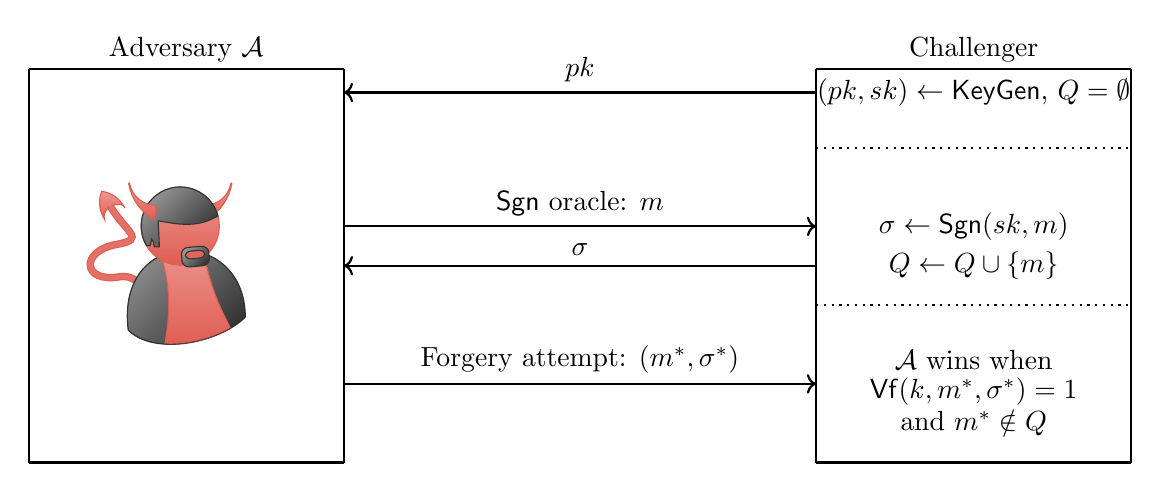
\begin{tikzpicture}
				
				\node[] (lblAdv) at (2,3.25) {Adversary $\mathcal{A}$};
				\draw[-,thick] (0,-2)--(4,-2);
				\draw[-,thick] (4,-2)--(4,3);
				\draw[-,thick] (4,3)--(0,3);
				\draw[-,thick] (0,3)--(0,-2);
				
				\node[devil, evil, minimum size=1.5cm] (Attacker) at (2,.5) {};
				
				\node[] (lblCha) at (12,3.25) {Challenger};
				\draw[-,thick] (10,-2)--(14,-2);
				\draw[-,thick] (14,-2)--(14,3);
				\draw[-,thick] (14,3)--(10,3);
				\draw[-,thick] (10,3)--(10,-2);
				
				\node[] (KeyGen) at (12,2.7) {$(pk,sk) \gets \mathsf{KeyGen}$, $Q = \emptyset$};
				\draw[<-,thick] (4,2.7) -- (10,2.7) node[midway,above] {$pk$};
				\draw[-, thick, dotted] (10,2) -- (14,2);
				
				\draw[->, thick] (4,1) -- (10,1) node[midway, above] {\textsf{Sgn} oracle: $m$};
				\node[] (Enc) at (12,1) {$\sigma \gets \mathsf{Sgn}(sk,m)$};
				\node[] (Add) at (12,.5) {$Q \gets Q \cup \{m\}$};
				\draw[<-,thick] (4,.5) -- (10,.5) node[midway, above] {$\sigma$};

				\draw[-,thick,dotted] (10,0) -- (14,0);
				
				\draw[->, thick] (4,-1) -- (10,-1) node[midway, above] {Forgery attempt: $(m^*, \sigma^*)$};
				\node[] (WinVfy) at (12,-.7) {$\mathcal{A}$ wins when};
				\node[] (WinVfy) at (12,-1.1) {$\mathsf{Vf}(k, m^*,\sigma^*) = 1$};
				\node[] (WinVfy) at (12,-1.5) {and $m^* \notin Q$};
				
			\end{tikzpicture}
\end{document}
